\documentclass[mathserif,handout]{beamer}
\usetheme{Warsaw}
\usecolortheme{seahorse}
\usecolortheme{orchid}
\usepackage{amsmath,verbatim}
\usepackage{listings}
\usepackage[english]{babel}
\usepackage{movie15}
\setbeamercovered{transparent}

\newcommand{\Deltap}{\ensuremath{\Delta^{\!+}}}
\newcommand{\trans}{\ensuremath{{}^\mathrm{T}}}
\newcommand{\eps}{\varepsilon}
\newcommand*{\approxdist}{\mathrel{\vcenter{\offinterlineskip
\vskip-.25ex\hbox{\hskip.55ex$\cdot$}\vskip-.25ex\hbox{$\sim$}
\vskip-.5ex\hbox{\hskip.55ex$\cdot$}}}}

% \lstMakeShortInline[language=myR]¬

\lstdefinelanguage{myR}
{
    language=R,
    otherkeywords={read.table, set.seed, Map},
    deletekeywords={url,codes, t, Call, formula,Q, R, on,by,hat,is,
col, set},
    sensitive=true,
    breaklines=true,
    morecomment=[l]{\#},
    morestring=[b]",
    morestring=[b]',
    basicstyle =\small\ttfamily,
    keywordstyle=\bf\color{blue},
    showtabs=false,
    showstringspaces=false,
    literate= {~}{$\sim$}{2},
    numberstyle=\sffamily\scriptsize,
    stepnumber=2
  }
\lstset{language=myR}

\title{Tempering MCMC}
\author[Darren Wilkinson --- SBSSB, 2/10/2013]{\textbf{\large Darren 
Wilkinson} \\
\alert{\url{http://tinyurl.com/darrenjw}}\\
School of Mathematics \& Statistics, \\
Newcastle University, UK}
\date{SBSSB Seminar\\Newcastle University\\2nd October, 2013}

\begin{document}

\frame{\titlepage}

\section{Introduction}

\subsection{Overview}

\frame{
\frametitle{Overview}
\begin{itemize}
\item Parallel tempering and MCMCMC
  \begin{itemize}
  \item Double well potential
  \item Parallel tempered chains
  \item Metropolis coupling of chains
  \item Blog post: \alert{\url{http://t.co/iFRjleKAhl}}
  \end{itemize}
\item Marginal likelihood from tempered Bayesian posteriors
  \begin{itemize}
  \item Tempered and power posteriors
  \item Marginal likelihood and normalising constants
  \item Bridge sampling and path sampling
  \item Blog post: \alert{\url{http://t.co/YMaa3Lz348}}
  \end{itemize}
\end{itemize}

{\small
Source code (R and \LaTeX\ of these slides):\\
\alert{\url{https://github.com/darrenjw/djwhacks/tree/master/r/temper}}}
}

\section{Parallel tempering and MCMCMC}

\subsection{Sampling a double well potential}

\frame{
\frametitle{Sampling a double-well potential}
 The simplest version assumes a potential function of the form
\[U(x) = \gamma (x^2-1)^2\]
for some given potential barrier height $\gamma$. The potential function $U(x)$ corresponds to the probability density function
\[\pi(x) \propto \exp\{-U(x)\}.\]
Think of potentials as being a (negative) log-density scale. On this scale, high potential barrier heights correspond to regions of very low probability density.
The point is that we have defined a multi-modal density, and that a Metropolis-Hastings algorithm initialised in one of the modes will have a hard time jumping to the other mode, and the difficulty of this jump will increase as we increase the value of $\gamma$.
}

\frame{
\frametitle{Potential function for $\gamma=4$}
\centerline{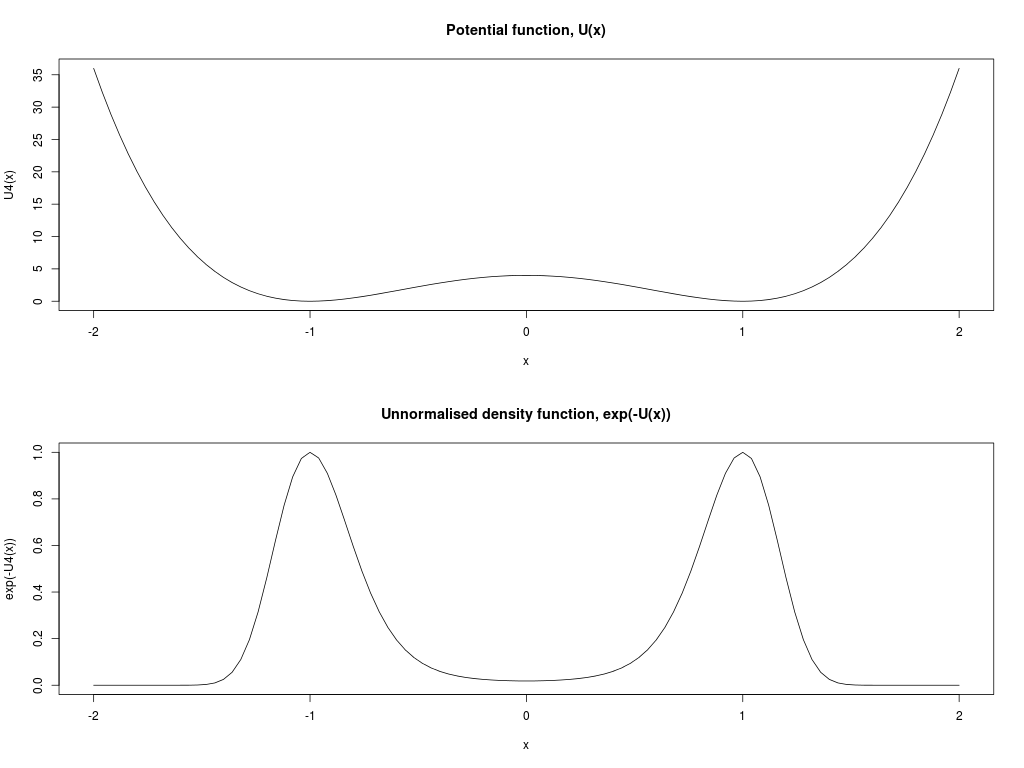
\includegraphics[height=0.8\textheight]{pot}}
}

\begin{frame}[fragile]
\frametitle{Sampling multiple chains in parallel}
\begin{lstlisting}
chains=function(pot=U, tune=0.1, init=1)
{
  x=rep(init,length(temps))
  xmat=matrix(0,iters,length(temps))
  for (i in 1:iters) {
    can=x+rnorm(length(temps),0,tune)
    logA=unlist(Map(pot,temps,x))-
             unlist(Map(pot,temps,can))
    accept=(log(runif(length(temps)))<logA)
    x[accept]=can[accept]
    xmat[i,]=x
  }
  colnames(xmat)=paste("gamma=",temps,sep="")
  xmat
}
mcmcSummary(chains(),rows=length(temps))
\end{lstlisting}
\end{frame}

\frame{
\frametitle{MCMC Output}
\centerline{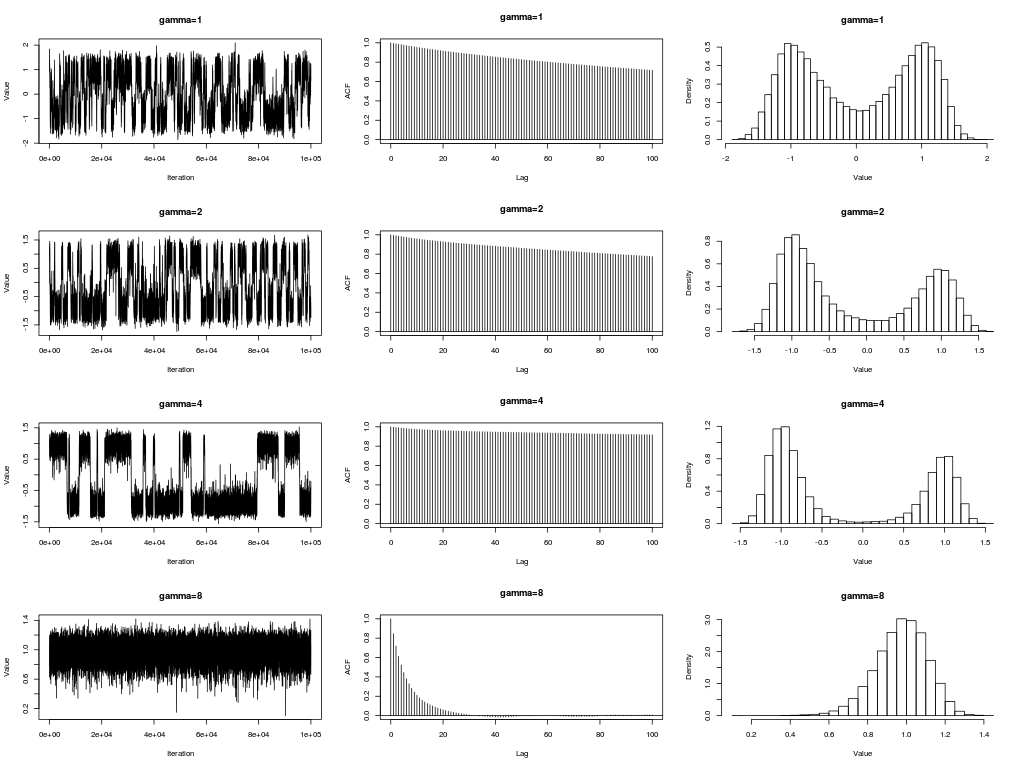
\includegraphics[height=0.8\textheight]{chains}}
}

\frame{
\frametitle{Analysis}

We see that as $\gamma$ increases, the chain jumps between modes less frequently. Indeed, for $\gamma=8$, the chain fails to jump to the second mode at all during this particular run of 100,000 iterations. That's a problem if we are really interested in sampling from distributions like this. Of course, for this particular problem, there are all kinds of ways to fix this sampler, but the point is to try and develop methods that will work in high-dimensional situations where we cannot just "look" at what is going wrong.
}

\subsection{Metropolis coupling of chains}

\frame{
\frametitle{Coupling parallel chains}
To keep things simple, let's just suppose that we have two (independent, parallel) chains, one with target $f(x)$ and the other with target $g(y)$. We can consider these chains to be evolving together, with joint target $\pi(x,y)=f(x)g(y)$. The updates chosen to update the within-chain states will obviously preserve this joint target. Now we consider how to swap states between the two chains without destroying the target. We simply propose a swap of $x$ and $y$. That is, we propose to move from $(x,y)$ to $(x^\star,y^\star)$, where $x^\star=y$ and $y^\star=x$, and therefore has density
\[q((x^\star,y^\star)|(x,y)) = \delta(x^\star-y)\delta(y^\star-x).\]
}

\frame{
\frametitle{Acceptance ratio}
As it is clearly a symmetric proposal it will drop out of the M-H ratio. Our acceptance probability is therefore $\min\{1,A\}$, where
\[\displaystyle A = \frac{\pi(x^\star,y^\star)}{\pi(x,y)} = \frac{\pi(y,x)}{\pi(x,y)} = \frac{f(y)g(x)}{f(x)g(y)}.\]
So, if we use this acceptance probability whenever we propose a swap of the states between two chains, then we will preserve the joint target, and hence the marginal targets and asymptotic independence of the target. However, the chains themselves will no longer be independent of one another. They will be coupled --- \alert{Metropolis coupled}.
}

\begin{frame}[fragile]
\frametitle{Sampling multiple chains in parallel}
\begin{lstlisting}
    .
    .
    accept=(log(runif(length(temps)))<logA)
    x[accept]=can[accept]
    # now the coupling update
    swap=sample(1:length(temps),2)
    logA=pot(temps[swap[1]],x[swap[1]])+pot(temps[swap[2]],x[swap[2]])-
            pot(temps[swap[1]],x[swap[2]])-pot(temps[swap[2]],x[swap[1]])
    if (log(runif(1))<logA)
      x[swap]=rev(x[swap])
    # end of the coupling update
    xmat[i,]=x
    .
    .
\end{lstlisting}
\end{frame}

\frame{
\frametitle{MCMC Output}
\centerline{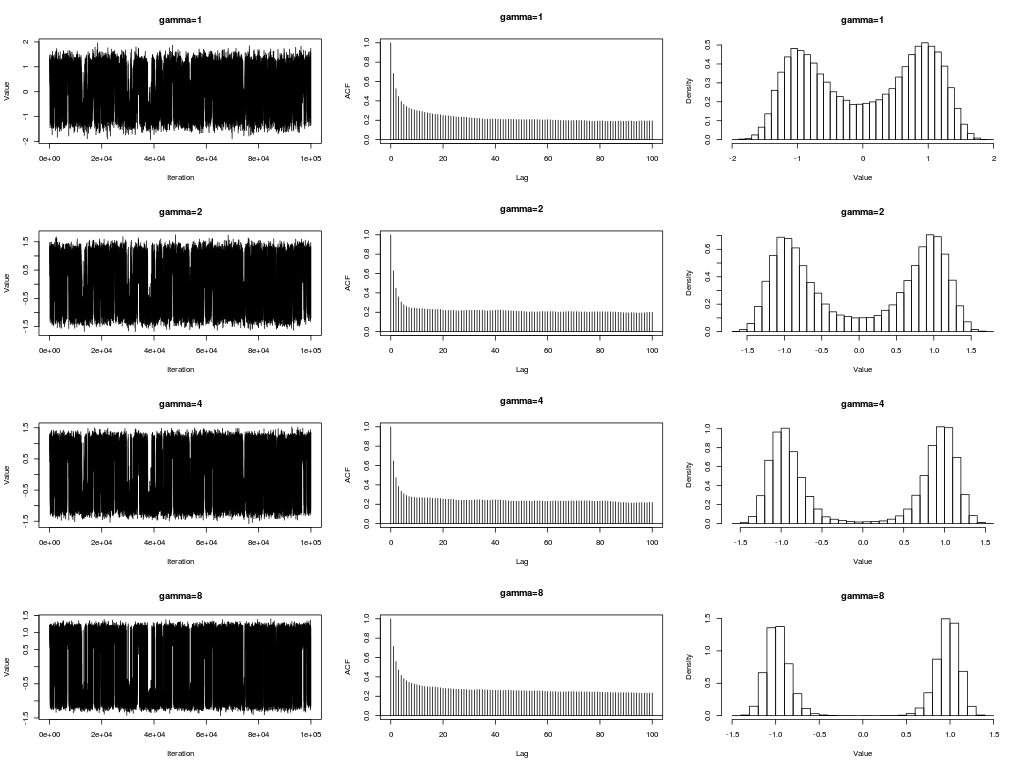
\includegraphics[height=0.8\textheight]{cchains}}
}

\frame{
\frametitle{Analysis}
We see immediately from the plots that whilst the individual target distributions remain unchanged, the mixing of the chains is \emph{greatly} improved (though still far from perfect). Note that in the code above I just picked two chains at random to propose a state swap. In practice people typically only propose to swap states between chains which are \alert{adjacent} - i.e. most similar, since proposed swaps between chains with very different targets are unlikely to be accepted. 
}

\frame{
\frametitle{Parallel implementation}
It should be clear that there are opportunities for parallelising the above algorithm to make effective use of modern multi-core hardware. An approach using \alert{\href{http://en.wikipedia.org/wiki/Openmp}{OpenMP}} with C++ is discussed in \alert{\href{http://www.lindonslog.com/programming/openmp/parallel-tempering-algorithm-c/}{this blog post}}. Also note that if the state space of the chains is large, it can be much more efficient to swap temperatures between the chains rather than states - so long as you are careful about keeping track of stuff - this is explored in detail in \alert{Altekar et al ('04)}.
}

\section{Marginal likelihood from tempered Bayesian posteriors}

\subsection{Tempering}

\frame{
\frametitle{Tempering Bayesian posteriors}
There are (at least) a couple of obvious ways that one can temper a Bayesian posterior distribution. Perhaps the most obvious way is a simple flattening, so that if
\[
\pi(\theta|y) \propto \pi(\theta)\pi(y|\theta)
\]
is the posterior distribution, then for $t\in [0,1]$ we define
\[
\pi_t(\theta|y) \propto \pi(\theta|y)^t \propto [ \pi(\theta)\pi(y|\theta) ]^t.
\]
This corresponds with the tempering that is often used in statistical physics applications. We recover the posterior of interest for $t=1$ and tend to a flat distribution as $t\longrightarrow 0$. 
}

\frame{
\frametitle{Power posterior}
However, for Bayesian posterior distributions, there is a different way of tempering that is often more natural and useful, and that is to temper using the \alert{power posterior}, defined by
\[
\pi_t(\theta|y) \propto \pi(\theta)\pi(y|\theta)^t.
\]
Here we again recover the posterior for $t=1$, but get the prior for $t=0$. Thus, the family of distributions forms a natural \alert{bridge} or \alert{path} from the prior to the posterior distributions. The power posterior is a special case of the more general concept of a geometric path from distribution $f(\theta)$ (at $t=0$) to $g(\theta)$ (at $t=1$) defined by
\[
h_t(\theta) \propto f(\theta)^{1-t}g(\theta)^t,
\]
where, in our case, $f(\cdot)$ is the prior and $g(\cdot)$ is the posterior.
}

\frame{
\frametitle{Parallel tempering}
So, given a posterior distribution that is difficult to sample, choose a \alert{temperature schedule}
\[
0=t_0<t_1<\cdots<t_{N-1}<t_N=1
\]
and run a parallel tempering scheme as outlined previously. The idea is that for small values of $t$ mixing will be good, as prior-like distributions are usually well-behaved, and the mixing of these "high temperature" chains can help to improve the mixing of the "low temperature" chains that are more like the posterior (note that $t$ is really an \emph{inverse} temperature parameter the way I've defined it here...).
}

\subsection{Marginal likelihood and normalising constants}

\frame{
\frametitle{Marginal likelihood}
The \alert{marginal likelihood} of a Bayesian model is
\[
\pi(y) = \int_\Theta \pi(\theta)\pi(y|\theta)d\theta.
\]
This quantity is of interest for many reasons, including calculation of the \alert{\href{http://en.wikipedia.org/wiki/Bayes_factor}{Bayes factor}} between two competing models. Note that this quantity has several different names in different fields. In particular, it is often known as the \alert{evidence}, due to its role in Bayes factors. It is also worth noting that it is the \alert{normalising constant} of the Bayesian posterior distribution. Although it is very easy to describe and define, it is notoriously difficult to compute reliably for complex models. 
}

\frame{
\frametitle{Importance estimator}
The normalising constant is conceptually very easy to estimate. From the above integral representation, it is clear that
\[
\pi(y) = E_\pi [ \pi(y|\theta) ]
\]
where the expectation is taken with respect to the prior. So, given samples from the \alert{prior}, $\theta_1,\theta_2,\ldots,\theta_n$, we can construct the Monte Carlo estimate
\[
\displaystyle \widehat{\pi}(y) = \frac{1}{n}\sum_{i=1}^n \pi(y|\theta_i)
\]
and this will be a consistent estimator of the true evidence under fairly mild regularity conditions.
}

\frame{
\frametitle{Bridge sampling}
Unfortunately, in practice it is likely to be a very poor estimator if the posterior and prior are not very similar. Now, we could also use Bayes theorem to re-write the integral as an expectation with respect to the posterior, so we could then use samples from the posterior to estimate the evidence. This leads to the \alert{harmonic mean estimator} of the evidence, which has been described as \alert{\href{http://radfordneal.wordpress.com/2008/08/17/the-harmonic-mean-of-the-likelihood-worst-monte-carlo-method-ever/}{the worst Monte Carlo method ever}}! 

Now it turns out that there are \emph{many} different ways one can construct estimators of the evidence using samples from the prior and the posterior, some of which are considerably better than the two I've outlined. This is the subject of the \alert{bridge sampling} paper of \alert{Meng and Wong ('96)}. However, the reality is that no method will work well if the prior and posterior are very different.
}

\frame{
\frametitle{Ratios of normalising constants}
If we have tempered chains, then we have a sequence of chains targeting distributions which, by construction, are not too different, and so we can use the output from tempered chains in order to construct estimators of the evidence that are more numerically stable. If we call the evidence of the $i$th chain $z_i$, so that $z_0=1$ and $z_N=\pi(y)$, then we can write the evidence in telescoping fashion as
\[
\displaystyle \pi(y)=z_N = \frac{z_N}{z_0} = \frac{z_1}{z_0}\times \frac{z_2}{z_1}\times \cdots \times \frac{z_N}{z_{N-1}}.
\]
Now the $i$th term in this product is $z_{i+1}/z_{i}$, which can be estimated using the output from the $i$th and/or $(i+1)$th chain(s). Again, this can be done in a variety of ways, using your favourite bridge sampling estimator. 
}

\frame{
\frametitle{Estimating ratios}
For the power posterior, the simplest method is to write
\begin{multline*}
\displaystyle \frac{z_{i+1}}{z_i} = \frac{\displaystyle \int \pi(\theta)\pi(y|\theta)^{t_{i+1}}d\theta}{z_i} \\= \int \pi(y|\theta)^{t_{i+1}-t_i}\times \frac{\pi(y|\theta)^{t_i}\pi(\theta)}{z_i}d\theta = E_i\left[\pi(y|\theta)^{t_{i+1}-t_i}\right],
\end{multline*}
where the expectation is with respect to the $i$th target, and hence can be estimated in the usual way using samples from the $i$th chain.
}

\frame{
\frametitle{Log evidence}
For numerical stability, in practice we compute the log of the evidence as
\begin{multline}
 \log\pi(y) = \sum_{i=0}^{N-1} \log\frac{z_{i+1}}{z_i} = \sum_{i=0}^{N-1} \log E_i\left[\pi(y|\theta)^{t_{i+1}-t_i}\right]\displaystyle \nonumber\\
= \sum_{i=0}^{N-1} \log E_i\left[\exp\{(t_{i+1}-t_i)\log\pi(y|\theta)\}\right].
\end{multline}
The above expression is exact, and is the obvious formula to use for computation. However, it is clear that if $t_i$ and $t_{i+1}$ are sufficiently close, it will be approximately OK to switch the expectation and exponential, giving
\[
\displaystyle \log\pi(y) \approx \sum_{i=0}^{N-1}(t_{i+1}-t_i)E_i\left[\log\pi(y|\theta)\right].
\]
}

\frame{
\frametitle{Path sampling}
In the continuous limit, this gives rise to the well-known \alert{path sampling identity},
\[
\displaystyle \log\pi(y) = \int_0^1 E_t\left[\log\pi(y|\theta)\right]dt.
\]
So, an alternative approach to computing the evidence is to use the samples to approximately numerically integrate the above integral, say, using the \alert{\href{http://en.wikipedia.org/wiki/Trapezoidal_rule}{trapezium rule}}. However, it isn't completely clear (to me) that this is better than using the exact sum directly.
}

\subsection{Example}

\frame{
\frametitle{Example: double well potential}
We can illustrate these ideas using the simple double potential well example from earlier. That example doesn't really correspond to a Bayesian posterior, and is tempered directly, rather than as a power posterior, but essentially the same ideas follow for general parallel tempered distributions. In general, we can use the sample to estimate the ratio of the last and first normalising constants, $z_N/z_0$. 

As before, we expand as a telescopic product, where the $i$th term is now
\[
\displaystyle \frac{z_{i+1}}{z_i} = E_i\left[\exp\{-(\gamma_{i+1}-\gamma_i)(x^2-1)^2\}\right].
\]
A Monte Carlo estimate of each of these terms is formed using the samples from the $i$th chain, and the logs of these are then summed to give $\log(z_N/z_0)$.
}

\begin{frame}[fragile]
\frametitle{Computing the evidence}
\begin{lstlisting}
mat=chains()
mat=mat[,1:(length(temps)-1)]
diffs=diff(temps)
mat=(mat*mat-1)^2
mat=-t(diffs*t(mat))
mat=exp(mat)
logEvidence=sum(log(colMeans(mat)))
message(paste("The log evidence is",logEvidence))
\end{lstlisting}
It works! The correct answer is approximately -1.12.
\end{frame}

\section{References}

\frame{
\frametitle{References}
{\scriptsize
\begin{itemize}
\item G. Altekar et al (2004) \alert{\href{http://dx.doi.org/10.1093/bioinformatics/btg427}{Parallel Metropolis coupled Markov chain Monte Carlo for Bayesian phylogenetic inference}}, Bioinformatics, 20(3): 407-415.
\item C. J. Geyer (2011) Importance sampling, simulated tempering, and umbrella sampling, in the \alert{\href{http://amzn.to/165vysu}{Handbook of Markov Chain Monte Carlo}}, S. P. Brooks, et al (eds), Chapman \& Hall/CRC.
\item C. J. Geyer (1991) \alert{\href{http://users.stat.umn.edu/geyer/f05/8931/c.pdf}{Markov chain Monte Carlo maximum likelihood}}, Computing Science and Statistics, 23: 156-163.
\item Meng, Xiao-Li, and Wing Hung Wong. "\alert{Simulating ratios of normalizing constants via a simple identity: a theoretical exploration}." Statistica Sinica 6.4 (1996): 831-860.
\item Gelman, Andrew, and Xiao-Li Meng. "\alert{\href{http://www.jstor.org/stable/2676756}{Simulating normalizing constants: From importance sampling to bridge sampling to path sampling}}." Statistical Science (1998): 163-185.
\item Friel, Nial, and Anthony N. Pettitt. "\alert{\href{http://dx.doi.org/10.1111/j.1467-9868.2007.00650.x}{Marginal likelihood estimation via power posteriors}}." Journal of the Royal Statistical Society: Series B (Statistical Methodology) 70.3 (2008): 589-607.
\item Friel, Nial, and Jason Wyse. "\alert{\href{http://dx.doi.org/10.1111/j.1467-9574.2011.00515.x}{Estimating the evidence --- a review}}." Statistica Neerlandica 66.3 (2012): 288-308.

\end{itemize}}
}



\end{document}

% eof


